\documentclass{beamer}

\setbeamerfont{framesubtitle}{size=\Large}
\setbeamerfont{frametitle}{size=\huge}


\usepackage{tikz}
\usepackage{verbatim}
\usepackage{listings}


\lstset
{ %Formatting for code in appendix
    language=Erlang,
    basicstyle=\scriptsize,
    numbers=left,
    xleftmargin=0.5cm,
    stepnumber=1,
    showstringspaces=false,
    tabsize=2,
    breaklines=true,
    breakatwhitespace=false,
}

\RequirePackage{polyglossia} 
\setdefaultlanguage{english}
\setotherlanguage{lithuanian}
\title{Pakartotinis kodo panaudojimas pirminio kriptovaliutų platinimo išmaniuosiuose kontraktuose}
\subtitle{Code Reuse in Initial Coin Offering Smart Contracts}
\author[shortname]{Agnė Mačiukaitė \and \\ Vadovas: lekt. Gediminas Rimša  }
\date{2018-06-25}

\addtobeamertemplate{frametitle}{}{
	\begin{tikzpicture}[remember picture,overlay]
	\node[anchor=north east,yshift=2pt] at (current page.north east) {
\includegraphics[height=1.5cm]{mif-logo.png}};
	\end{tikzpicture}}

\setbeamertemplate{footline}[text line]{%
	\parbox{\linewidth}{\vspace*{-12pt}\hfill\insertpagenumber/\inserttotalframenumber}}
\setbeamertemplate{navigation symbols}{}


\begin{document}

	
\maketitle


\section{Tematika}

\subsection{}
\begin{frame}{\insertsection}
\framesubtitle{\insertsubsection}
    \vspace{-35.5pt}
\begin{itemize}
	\item Pakartotinis kodo panaudojimas:
    \begin{itemize}
        \item Produktų linijos;
        \item Savybių modeliavimas.
    \end{itemize}

    \item Išmanieji kontraktai:
	\begin{itemize}
        \item Blockchain;
        \item Pirminis kriptovaliutų platinimas (angl. initial coin offering (ICO)).
    \end{itemize}
\end{itemize}
\end{frame}


\section{Tikslas ir uždaviniai}
\begin{frame}{\insertsection}
	\framesubtitle{\insertsubsection}
    \vspace{-35.5pt}
	\setlength\parindent{20pt}\textbf{Tikslas}\\
    
    Ištirti pirminio finansavimo kriptovaliutomis išmaniuosius kontraktus, nustatyti, kokios savybės yra pastovios, o kokios - kintamos bei pasiūlyti būdus kodo pernaudojamumui didinti. 
    
  
    \textbf{Tikslui pasiekti išsikelti uždaviniai:}
    \begin{enumerate}
        \item Apžvelgti savybių modeliavimą programinės įrangos produktų linijos sričiai;
        \item Surinkti virš 100 išmaniųjų kontraktų skirtų ICO;
        \item Išskirti surinktų išmaniųjų kontraktų savybes;
        \item Sukurti ICO savybių modelį ir jį validuoti.
    \end{enumerate}
\end{frame}

\section{Savybių modeliavimas}
\subsection{Savybė}

\begin{frame}{\insertsection}
\framesubtitle{\insertsubsection}
\vspace{-20.5pt}
    \begin{itemize}
        \item Savybė -  pastebima ir skiriama sistemos charakteristika, kuri yra matoma įvairioms suinteresuotoms šalims;
        \item Savybės yra programinės įrangos atributai, kurie tiesiogiai paveikia
        naudotoją.
    \end{itemize}

\end{frame}


\begin{comment}
\end{comment}

\subsection{Savybių modelis}
\begin{frame}{\insertsection}
\framesubtitle{\insertsubsection}
\vspace{-20.5pt}
\begin{itemize}
    \item Savybių modelis - modelis, kuris turi pavaizduoti standartines sistemos šeimos savybes srityje ir santykius tarp jų;
\end{itemize}

\bigbreak
\bigbreak

\centering{Santykiai tarp savybių}
\begin{figure}[H]
    \centering
    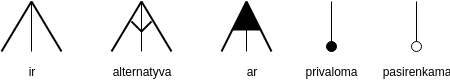
\includegraphics[scale=0.5]{../img/feature_model_rules}
%    \caption{}
    
\end{figure}
\end{frame}

\section{ICO savybių modeliavimas}
\subsection{ICO išmanieji kontraktai}
\begin{frame}{\insertsection}
	\framesubtitle{\insertsubsection}
    \vspace{-40.5pt}
    \begin{itemize}
        \item ICO išmaniųjų kontraktų surinkimas;
        \item ICO išmaniųjų kontraktų pasirinkimas savybių modeliavimui.
    \end{itemize}
	
\end{frame}



\subsection{ICO savybės}
\begin{frame}[fragile]{\insertsection}
	\framesubtitle{\insertsubsection}
    \begin{enumerate} 
        \item Minimalaus investavimo kriterijus;
        \item Kainos už žetoną pakeitimas;
        \item Kontrakto savininko nustatymas bei kai kurio funkcionalumo priskyrimas tik jam;
        \item Galimybė sustabdyti ICO ir vėl paleisti iš naujo;
        \item Pirkimas tik indentifikuotiems naudotojams;
        \item ICO pradžios nustatymas;
        \item Nustatytas maksimalus galimas žetonų kiekis nupirktas per kartą;
        \item Nereikalingų žetonų išsitraukimas iš kontrakto.
    \end{enumerate}
\end{frame}


\subsection{ICO savybių modelis}
\begin{frame}{\insertsection}
	\framesubtitle{\insertsubsection}
    \vspace{-35.5pt}
	\begin{figure}[H]
		\centering
		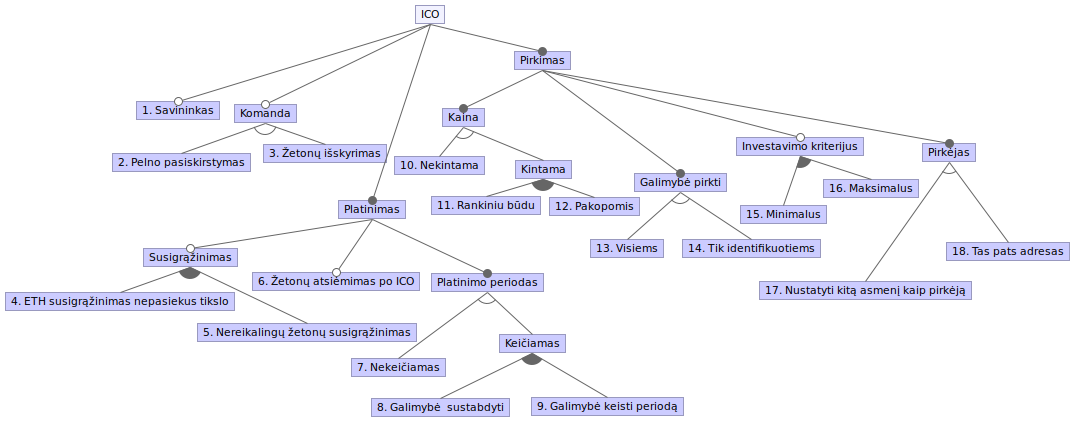
\includegraphics[scale=0.3]{../img/ico_model_num}


	\end{figure}
\end{frame}

\subsection{ICO savybių modelis}
\begin{frame}{\insertsection}
\framesubtitle{\insertsubsection}
\vspace{-35.5pt}
 ICO savybių modelio kompozicijos taisyklės:
    \begin{enumerate}
        \item Nereikalingų žetonų susigrąžinimui reikalingas savininkas;
        \item Platinimo periodo keitimui reikalingas savininkas;
        \item Kainos pakeitimui rankiniu būdu reikalingas savininkas;
        \item Žetonus atsiimti po ICO gali tik pirkėjas;
        \item ETH susigrąžinti nepasiekus tikslo gali tik pirkėjas.
    \end{enumerate}
\end{frame}


\subsection{ICO savybių modelio validacija}
\begin{frame}{\insertsection}
\framesubtitle{\insertsubsection}
\vspace{-35.5pt}
\begin{itemize}
    \item Validacijos metodas;
    \item Validacijos procesas;
    \item Validacijos rezultatas.
\end{itemize}

\end{frame}


\section{Rezultatai ir išvados}

\begin{frame}
	\frametitle{Rezultatai}
	\begin{enumerate}
        \item Apžvelgtos kodo pernaudojimo galimybės naudojantis savybių modeliavimu;
        \item Surinkti ICO išmanieji kontraktai bei ištirtos jų savybės;
        \item Nustatyta, kurios savybės yra pastovios ir kintamos;
        \item Kodo pernaudojamumui didinti sudarytas savybių modelis.
	\end{enumerate}
\end{frame}

\begin{frame}
	\frametitle{Išvados}
	\begin{enumerate}
        \item Savybių modeliavimas yra geras būdas ICO išmaniųjų kontraktų kodo pernaudojamumui didinti;
        \item Yra sukurta pakankamai daug ICO išmaniųjų kontraktų turinčių įvairių savybių, todėl žinant, koks savybių rinkinys yra reikalingas, būtų galima pernaudoti esamą kontraktą ar jo dalį.
	\end{enumerate}
\end{frame}
\end{document}